Utilizamos os dados de casos confirmados de COVID-19 e de mortes causadas pela doença do município do Rio de Janeiro que podem ser encontrados no site da prefeitura do Rio de Janeiro \cite{data-rio-covid} e servem de base para o Painel Rio COVID-19 \cite{painel-rio-covid}, com atualização diária. 
Na captura de dados, podemos encontrar uma série de dificuldades relacionadas ao rastreio de casos, tais como a baixa testagem na cidade, o atraso na notificação e os ciclos semanais causados pela forma como são feitos os registros. 
Esses fatores dificultam o processo de aprendizado sobre os parâmetros. 

A partir da obtenção e tratamento desses dados, podemos obter a curva do número de indivíduos infectados confirmados que declaram início dos sintomas no tempo $t$, representado pela curva $T$ no nosso modelo, e também o dia de morte, o que permite recuperar a curva $D$. 
Está claro que pessoas podem informar a data de início dos sintomas com uma imprecisão de alguns dias, mas assumimos que esses erros são independentes, como explicado na Seção \ref{parameters}. 
A análise de dados mais detalhada pode ser conferida no repositório do Github \cite{github}.

\subsection{Análise de dados}
\label{data-analysis}

Após a obtenção dos dados em formato {\it CSV}, observamos que os dados como na Tabela \ref{tab:data-covid-rio}. 
A data de início de sintomas indica o dia que o paciente reportou ter começado a sentir os sintomas e a data de evolução marca o dia em que a pessoa se recupera ou falece e deixa de ser um caso ativo. Essa coluna é a que mais possui campos vazios (em torno de 6\%), em que apenas dois eram indivíduos com óbito confirmado e os outros se dividiam entre recuperados e ativos. 
As outras colunas são auto-explicativas e não terão atenção nesse trabalho.

\begin{table}
    \centering
    \resizebox{\textwidth}{!}{%
    \begin{tabular}{llllllllll}
        \toprule
        {} & dt\_notific & dt\_inicio\_sintomas & bairro\_resid\_estadia & ap\_residencia\_estadia & sexo & faixa\_etaria & evolucao & dt\_evolucao &  raca\_cor \\
        \midrule
        0 &   09/18/20 &           09/03/20 &            PACIENCIA &                   5.3 &    M &   De 50 a 59 &    OBITO &    09/17/20 &     Preta \\
        1 &   11/25/20 &           11/02/20 &      BARRA DA TIJUCA &                   4.0 &    M &   De 80 a 89 &    OBITO &    12/01/20 &    Branca \\
        2 &   05/06/20 &           05/06/20 &             CACHAMBI &                   3.2 &    M &   De 70 a 79 &    OBITO &    05/07/20 &  Ignorado \\
        3 &   11/12/20 &           11/02/20 &      BARRA DA TIJUCA &                   4.0 &    M &   De 70 a 79 &    OBITO &    12/12/20 &    Branca \\
        4 &   06/13/20 &           04/26/20 &      MARECHAL HERMES &                   3.3 &    M &   De 60 a 69 &    OBITO &    05/16/20 &  Ignorado \\
        \bottomrule
    \end{tabular}%
    }
    \caption{Cinco casos confirmados e os dados individuais: data de notificação, data de inicío dos sintomas, bairro de residência, área de planejamento em saúde, sexo, faixa etária, evolução, data de evolução e raça.}
    \label{tab:data-covid-rio}
\end{table}

Podemos visualizar a quantidade de novas notificações diariamente na Figura \ref{new-notifications}. 
Uma das características da curva em azul é a existência de uma grande variabilidade semanal, como afirmado no início da seção e, por esse esse motivo, como descrito na Seção \ref{moving-average}, é visualizada a curva da média de 7 dias em vermelho. 
Na Figura \ref{notifications-vs-symptoms}, comparamos as curvas médias de novas notificações e de indicações de início dos sintomas. 
Por exemplo, observamos que o primeiro pico do início dos sintomas não é repercutido na média de notificações (apesar de sabermos que a integral em todo o percurso é a mesma). Isso mostra que existe uma distribuição de quando as pessoas começam a sentir os sintomas a partir da infecção e de quando elas são notificadas pelo sistema. 

\begin{figure}[!ht]
    \centering
    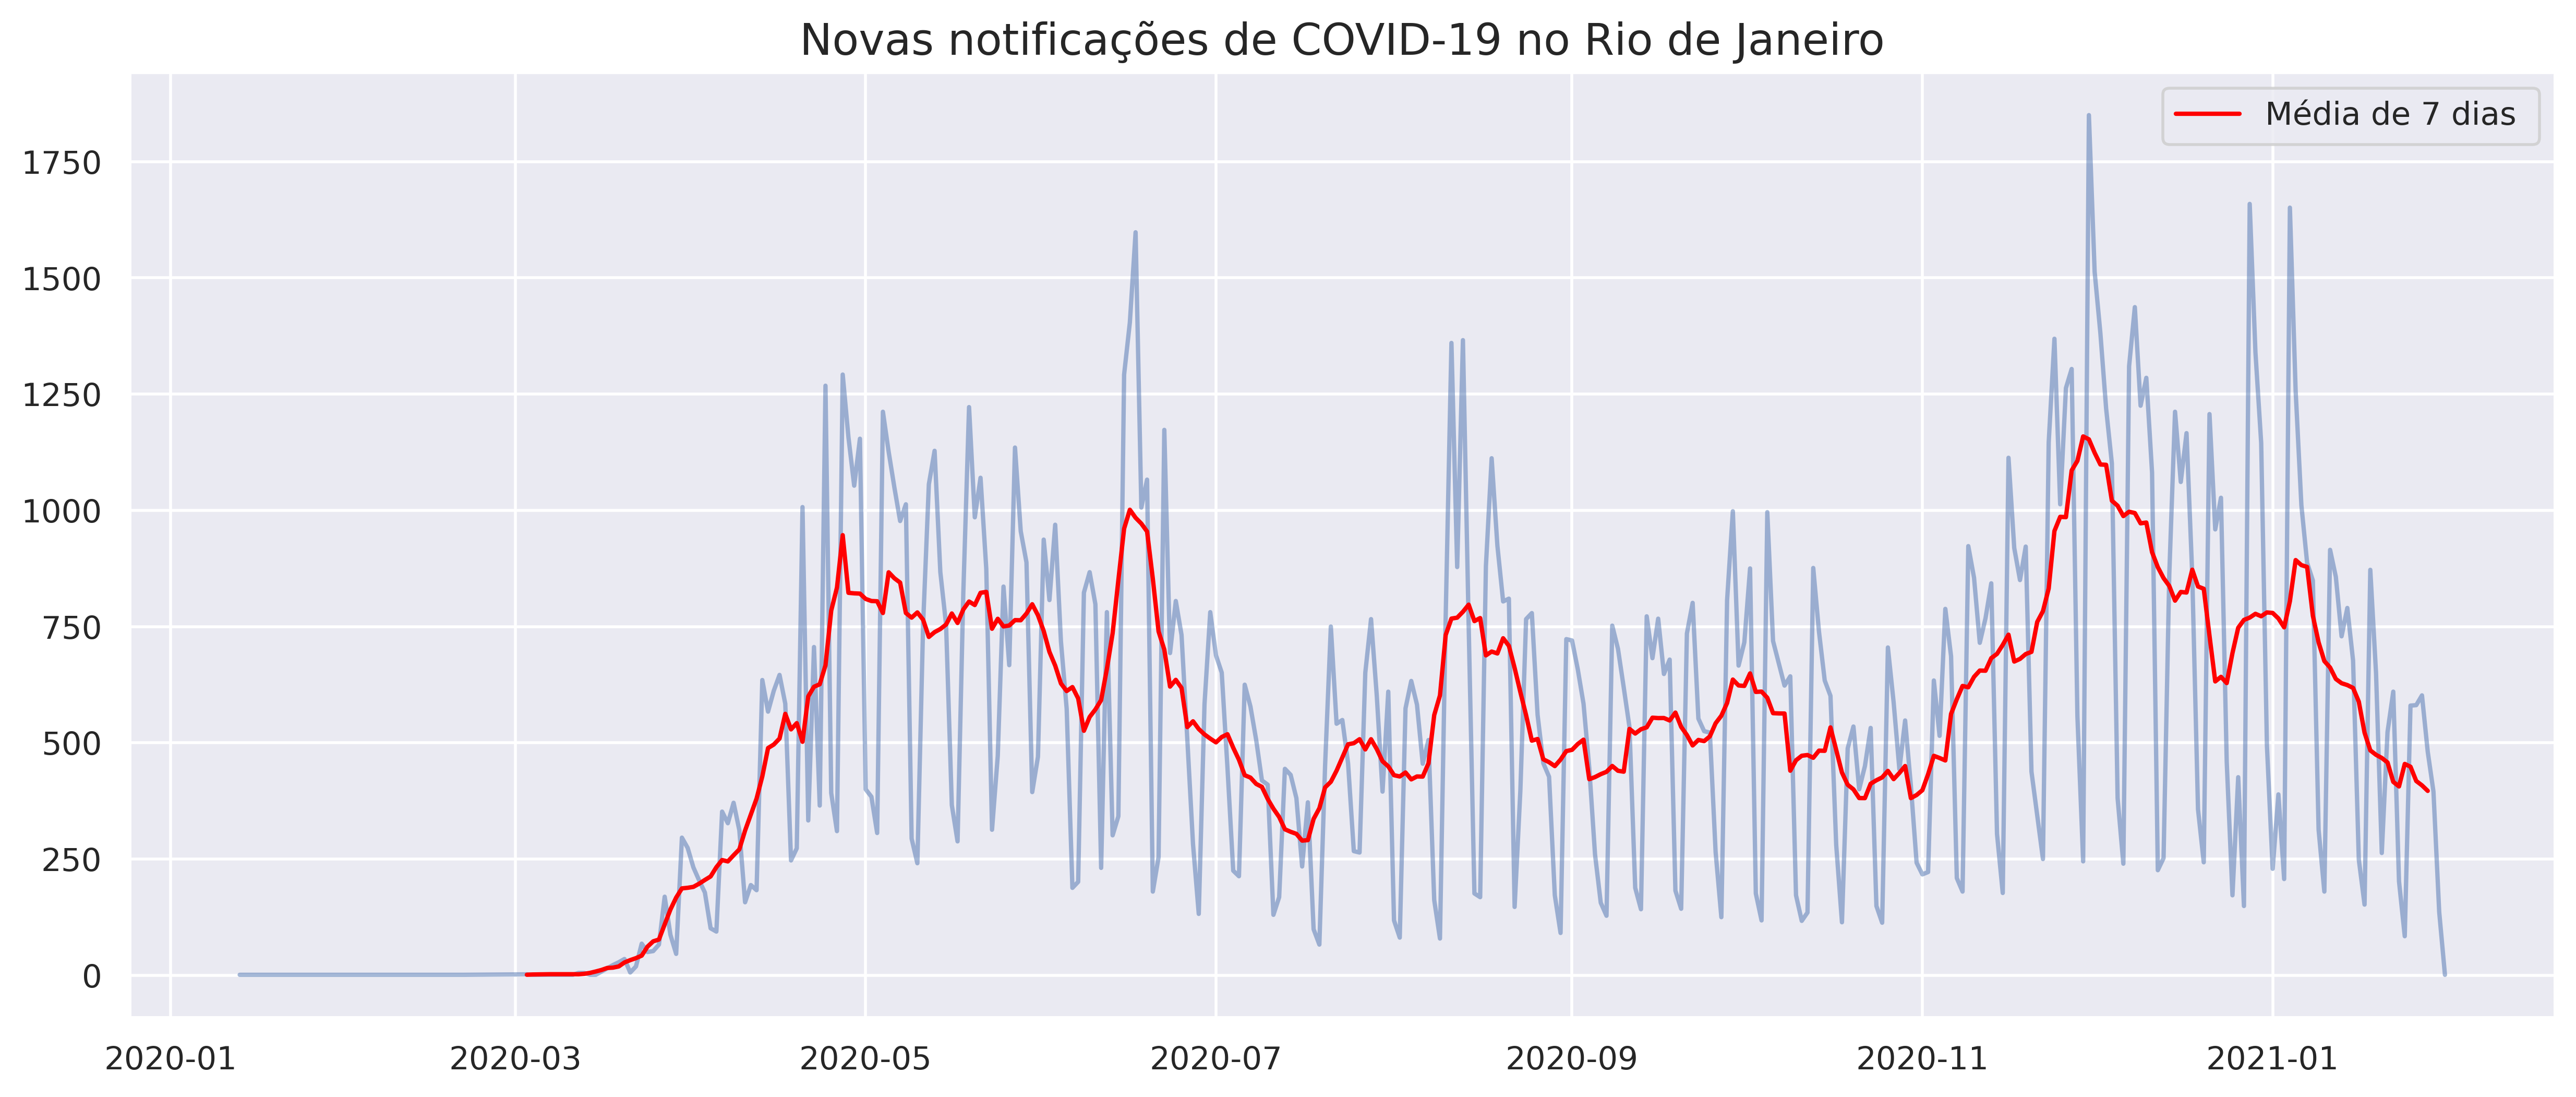
\includegraphics[width = \textwidth]
    {../images/new-notifications-rio.png}
    \caption{Notificações a cada dia ao longo da pandemia no Rio de Janeiro.}
    \label{new-notifications}
\end{figure}

\begin{figure}[!ht]
    \centering
    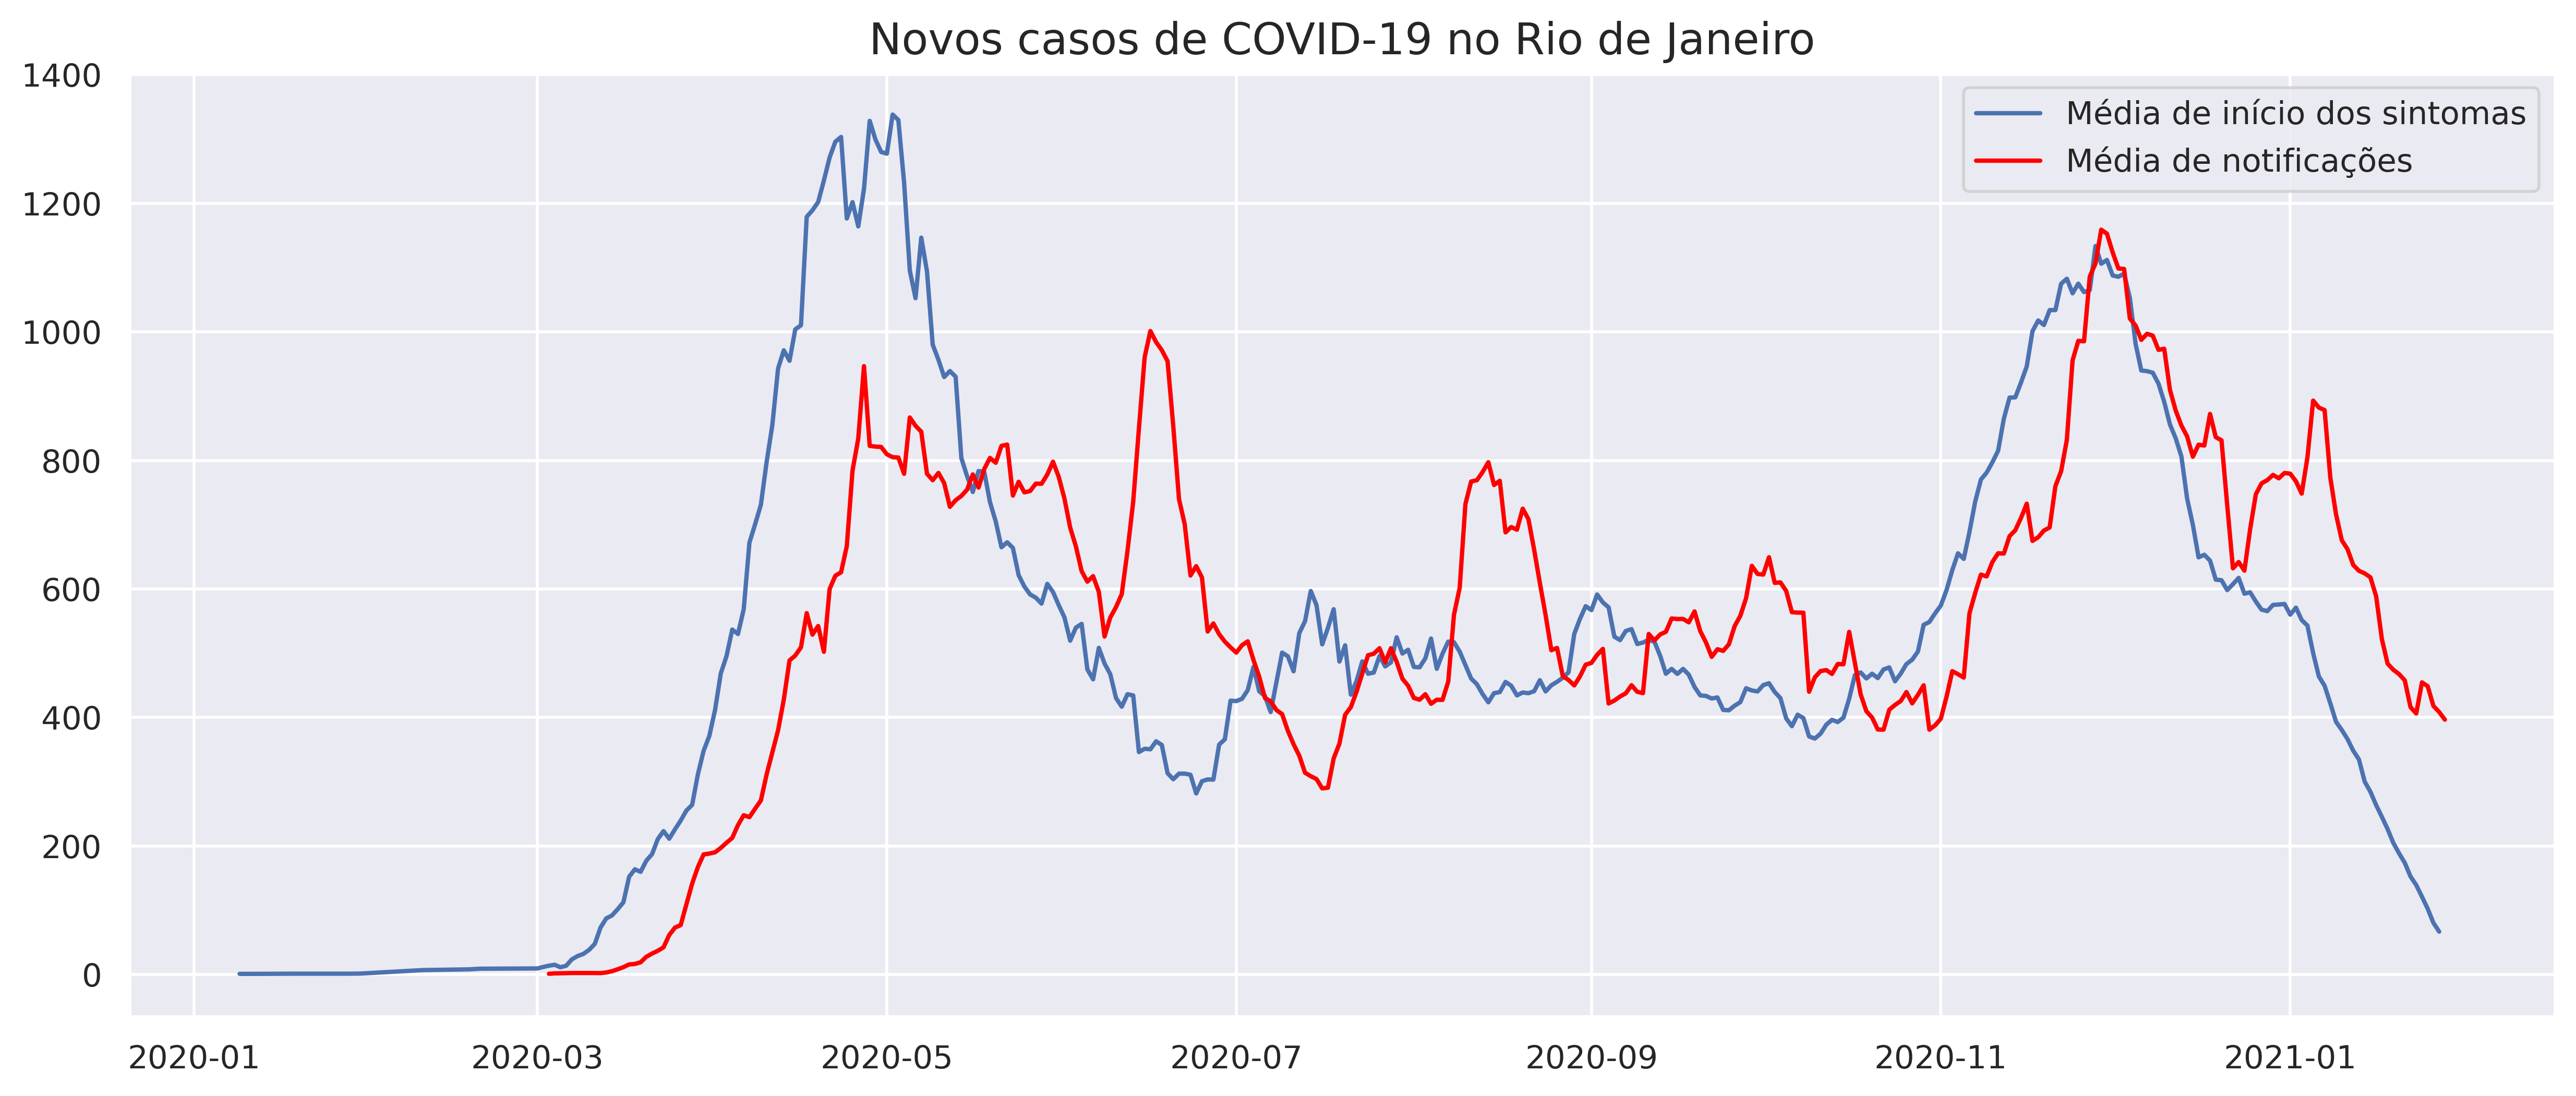
\includegraphics[width = \textwidth]{../images/comparing-symptoms-notifications.png}
    \caption{Comparação das curvas de média de 7 dias de novas notificações e indicação de início dos sintomas.}
    \label{notifications-vs-symptoms}
\end{figure}

Em agosto, o pico na média de notificações não é antecipado por um pico na curva de sintomas, isto é, as pessoas que notificaram esse mês devem ter começado a sentir os sintomas em um período anterior. 
Isso sugere que a curva em azul (média por início dos sintomas) é melhor a ser analisada, pois não sofre pelos problemas de atraso e inconstância. 
No final dessa curva, existe um decréscimo que não faz sentido com o pico anterior, pois as pessoas que indicarão o início dos sintomas nesse período vão ser notificadas nas semanas seguintes. 

Essa diferença de quando uma pessoa foi notificada e quando ela sentiu os primeiros sintomas pode ser visualizada em formato de histograma na Figura \ref{histogram-diff}. 
É importante destacar que valores negativos são claramente erros de digitação ou informação nos dados, como pôde ser examinado que existiam casos que foram notificados em 2021, mas com início dos sintomas em janeiro de 2020. 
Apesar disso, esses erros são em menor quantidade quando comparados à massa de dados. 
Registrou-se que em torno de 19,34\% dos dados têm tempo de notificação maior do que 30 dias e em torno de 1,29\% maior de 100 dias o que indica o grande atraso nas notificações.

\begin{figure}[!ht]
    \centering
    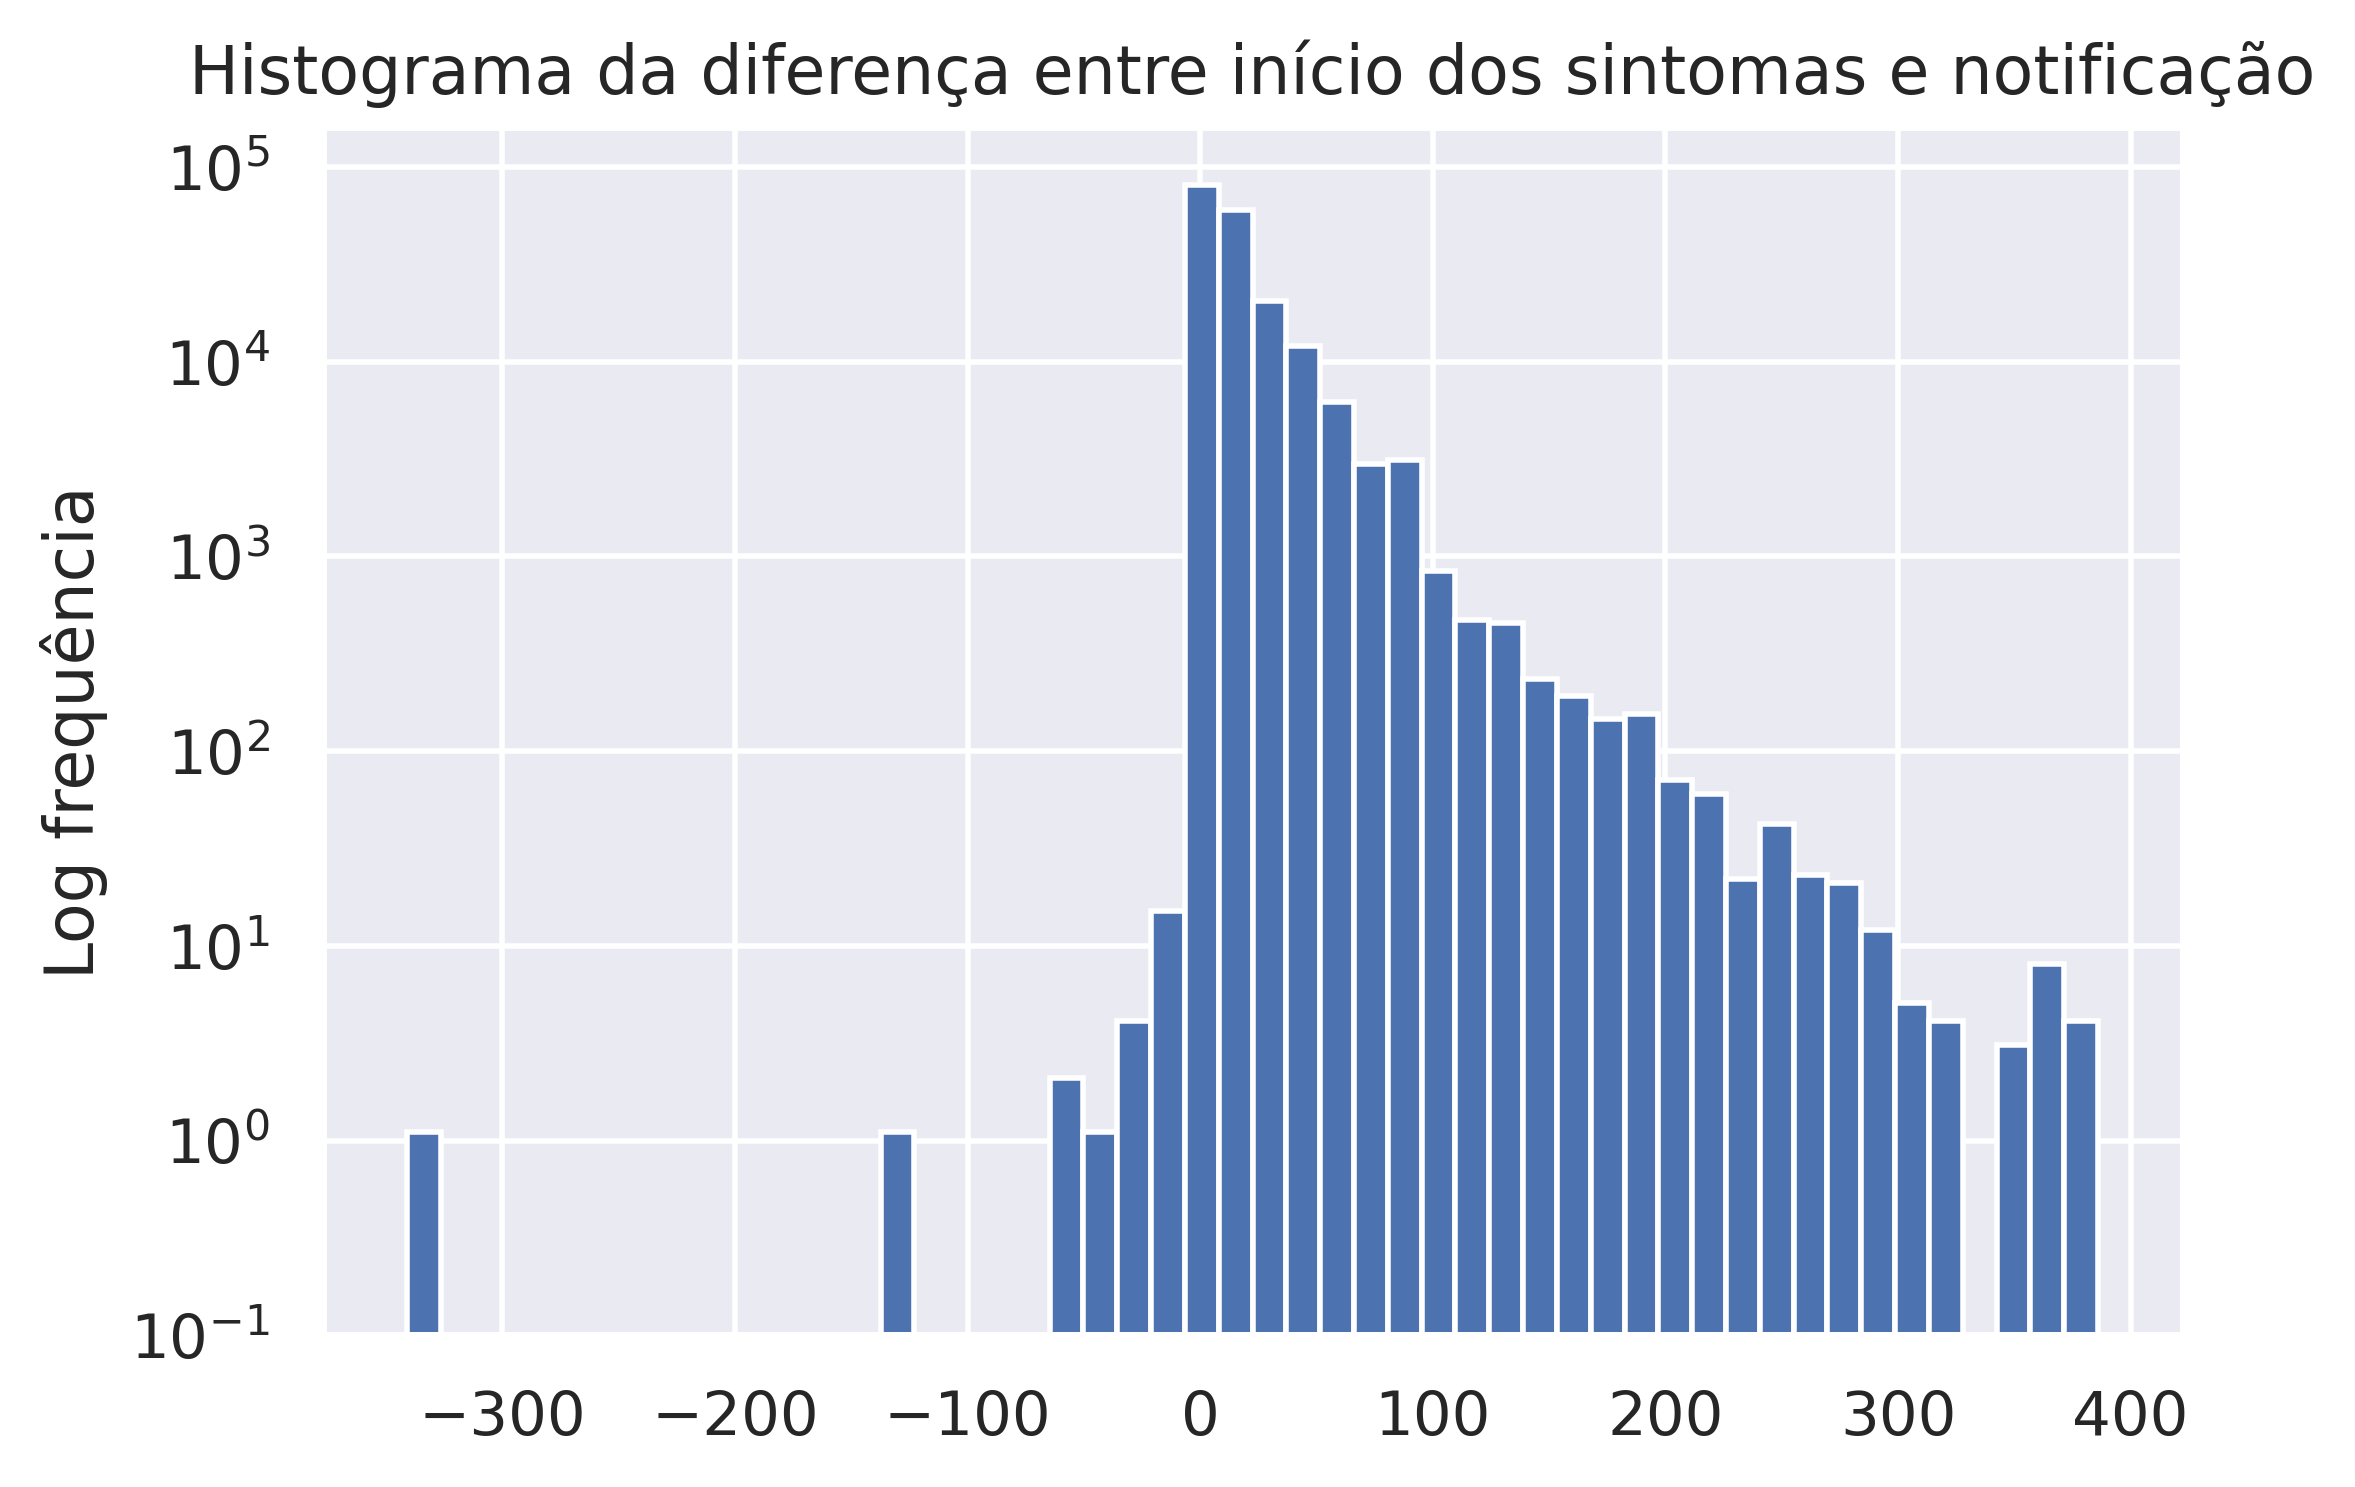
\includegraphics[width = .7\textwidth]{../images/histogram-comparion.png}
    \caption{Histograma da diferença entre o dia de notificação e o dia de início dos sintomas.}
    \label{histogram-diff}
\end{figure}

Uma análise com relação aos dados faltantes com comparação aos bairros, faixa etária e sexo também foi feita e pode ser vista no Github, mas apresentou pouca evidência para contribuir nesse trabalho. 
O mesmo tipo de exame pode ser feito para a evolução dos casos de óbitos, como pode ser visualizado na Figura \ref{deaths}. 
Muitos casos de mortes tiveram sua notificação a posteriori também, e omitimos o gráfico por razões de similaridade com o histograma anterior.
Por fim, para os campos com dados faltantes em data de início de sintomas e data de evolução daqueles com óbito registrado, houve uma imputação aleatória baseada na distribuição dos histogramas correspondentes. 

\begin{figure}[!ht]
    \centering
    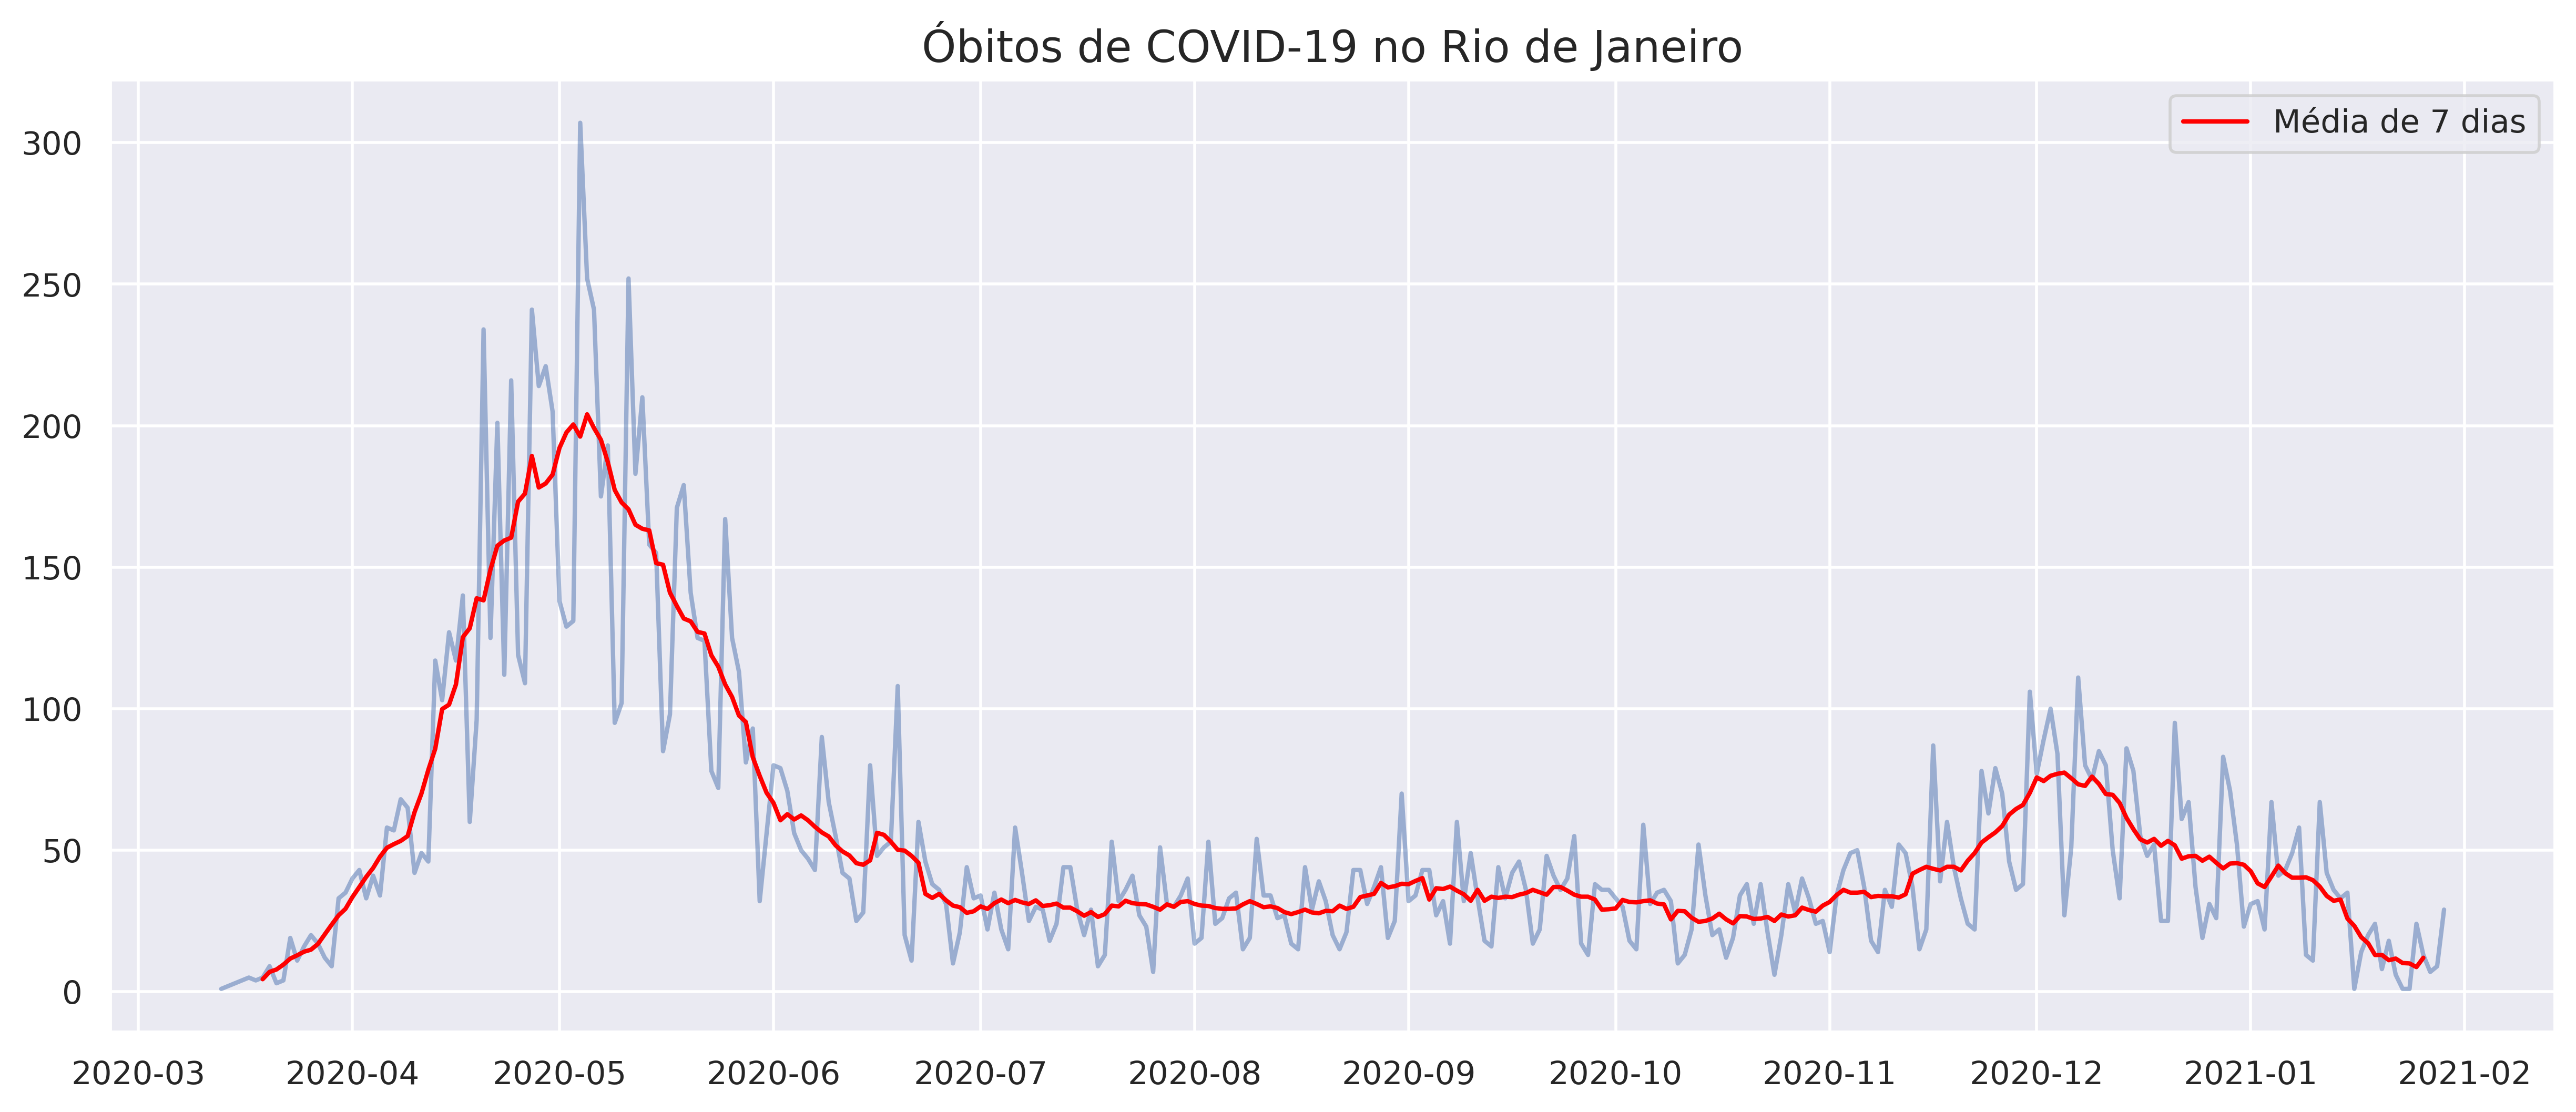
\includegraphics[width = \textwidth]{../images/deaths-rio.png}
    \caption{Evolução de óbitos no Rio de Janeiro.}
    \label{deaths}
\end{figure}

\subsection{Suavização das curvas}
\label{moving-average}

Constatamos ao longo do surto que existe uma sazonalidade semanal nos casos confirmados e de mortes, dado que nos fins de semana há um desvio negativo, enquanto na terça-feira um positivo. 
Essa variação semanal prejudica o modelo, pois ele não possui ajuste sazonal e, por esse razão, a aplicação de um suavizador se faz necessária. 
Nesse sentido, utilizaremos uma {\em média móvel} centrada com 7 dias.
Desta forma, se  $\{x_s\}_{1 \le s \le n}$ são nossos dados iniciais, estamos interessados em
\begin{equation}
    \hat{x}_t = \frac{1}{2k + 1}\sum_{s=-k}^k x_{t+s},
\end{equation}
em que $2k + 1 = 7$. Essa escolha é arbitrária, mas deriva diretamente da problemática semanal.

\subsection{Dados acumulados}

Por fim, obtemos as curvas acumuladas de novos casos e óbitos, a fim de
comparar com as curvas do modelo $T$ e $D$. Dessarte, nosso dado será da
forma
\begin{equation}
    y_t = \sum_{i=-14}^t \hat{x}_i, ~~~~(t = 0, ..., n)
\end{equation}